% Sample file on how to use subfiles.
\documentclass[ExampleMasters.tex]{subfiles}

\begin{document}
\clearpage
\chapter{Verification and validation of steering  (2-3 Seiten)}
\label{chap:testing}

\section{Overview}
In different states of the project different kind of tests were performed. As a first step bench tests were done to verify the developed software. Following that, several tests on the actual dolly, with the dolly in standstill and no trailers connected, were made.

\section{Bench-Testing}
\label{sec:bench-testing}
\subsection{ECU-setup}
\subsection{VTM maneuver verification}
\begin{itemize}
	\item include simulation results for maneuver of controller being run inside VTM
	\item perhaps include some picture of the video-output, with the actuated truck
	\item plots for maneuver (steering input, speed over time)
	
\end{itemize}
\subsection{CAN verification}
\begin{itemize}
	\item check output from ASF with arduino
	\item check ECU CANs, make sure they differ in output
	
\end{itemize}

\subsection{Fault detection system verification}
\label{sec:fault_detect_test}

\begin{itemize}
	\item send faulty inputs
	\item show plot of faulty input and system reaction
	
\end{itemize}
\section{Processing time evaluation}
\label{chap:processing_time_delay}
\subsection{Background}
The desired solution is supposed to operate at any speed. For high speeds a quick processing and transmission time is required to ensure prompt and realtime intervention of the control system based on the measured input signals. If the delays induced by the different components in the complete system are known or can be estimated, they can be compensated for in the steering-algorithm running on the rapid-prototyping system.

As outlined in section \ref{sec:measurement_setup} the dolly is equipped with a system to determine the deflection angle of the draw-bar and both the kingpin angles of the LVC. The sensors' raw signal is then parsed and filtered in an integrated low-level system which feeds the filtered signals to a private CAN-bus, where it is picked up by the MABII. The filtering operation takes a certain time and thus induces a delay. Furthermore the model running on the rapid-prototyping system needs a certain time to calculate the current desired steering angle for the dollys' wheels. This has to be determined as well. The steering mechanisms on the dolly are also a delay-inducer due to the inertia in the hydro-mechanic system. This is as well unavoidable, but when measured can as well to a certain degree be compensated for. 

The measuring chain for the logging solution will also be discussed and the different delays will be discussed. 

\subsection{Measured input delay}
\label{sec:measuring_delay}

The response time of the dolly's steering system was determined in workshop environment in stand-still without any additional axle loads. Tests were conducted for both axles individually to ensure that maximum power was available preventing further delays through insufficient electrical power or hydraulic pressure. A repeated steering angle in the form of a step input was used to determine the reaction time of the system. The step amplitude was increased over different tests to account for possible dependencies on articulation of the steering system. The tests each started and ended with a steering angle of $0^\circ .$ An example for the test sequence can be seen in figure \ref{fig:example_for_step_input_delay_measuring}. Clearly the difference between the requested angle and the actual articulation of the wheel can be seen. Further discussion of the results can be found in section \ref{sec:results_processing_time}.\\

\begin{figure*}
\centering
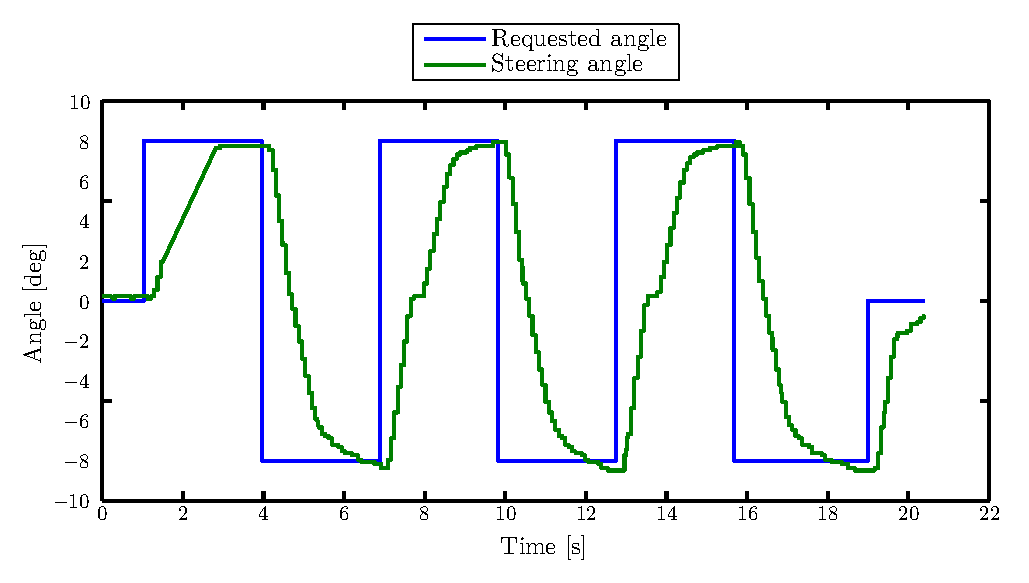
\includegraphics[width=1\linewidth]{figures/example_for_step_input_delay_measuring}
\caption{Example of step input for delay determination, front axle lifted, $8^\circ $ amplitude, six repetitions.}
\label{fig:example_for_step_input_delay_measuring}
\end{figure*}


To eliminate tire friction the investigated axle was suspended in the air in further series of testing by slightly craning up the dolly's front/rear (see figure \ref{fig:dolly_craned_up}) to allow for free movement of the tires. An example for the utilized testing routine can be gathered from table \ref{tab:test_matrx_delay_measuring}. Between the different steps (double amplitude) a sufficient wait time of 3500ms was used to allow the system to reach the requested steering angle. This waiting time was kept constant throughout all tests. \\

	\begin{table}[h]
		\label{tab:test_matrx_delay_measuring}
		\centering
		\begin{tabular}{llll}
			\textbf{\#} & \textbf{Amplitude [$  ^\circ $]} & \textbf{Axle}  & \textbf{Comment}                                                                  \\
			1  & 1                & front & lift front axle, ETS dead band \\
			2  & 2                & front &                                                                          \\
			3  & 3                & front &                                                                          \\
			4  & 4                & front &                                                                          \\
			5  & 5                & front &                                                                          \\
			6  & 6                & front &                                                                          \\
			7  & 7                & front &                                                                          \\
			8  & 8                & front &                                                                          \\
			9  & 9                & front & error mode, step too\footnotemark[1]                                      \\\hline
			10 & 1                & rear  & lift rear axle, ETS dead band  \\
			11 & 2                & rear &                                                                          \\
			12 & 3                & rear &                                                                          \\
			13 & 4                & rear &                                                                          \\
			14 & 5                & rear &                                                                          \\
			15 & 6                & rear &                                                                          \\
			16 & 7                & rear &                                                                          \\
			17 & 8                & rear &                                                                          \\
			18 & 9                & rear & error mode, step too big\footnotemark[1]                                                                   \\
			
		\end{tabular}
		\caption{Test matrix for delay measuring with lifted axle (analogous matrix for non-lifted testing (\#19-\#36))}
	\end{table}
	\footnotetext[1]{If a too big of a step is requested from the steering system, VSE's ECU will go into emergency mode. Steering is completely locked, turning the dolly completely passive.}   


As also described in section \ref{sec:results_processing_time} additional response tests were conducted utilizing a ramp input. Here a maximum steering amplitude of $15^\circ $ was used and the slope of the ramp was varied. As the request was not in the form of a step input, no error was triggered like in test \#9 and \#18 (see table \ref{tab:test_matrx_delay_measuring}). The test matrix for this setup is outlined in table \ref{tab:test_matrx_ramp_input}. 

\begin{table}[h]
	\label{tab:test_matrx_ramp_input}
	\centering
\begin{tabular}{llllll}
 \textbf{\#} &\textbf{ Amplitude [$^\circ$]} & \textbf{Rate} & \textbf{Sample time [s]} & \textbf{Comment} &  \\ 
1	  &  15 & 0.01 & 0.001 &   \\ 
2	  & 15 & 0.001 &  0.001&  \\ 
3	  & 15 & 0.1 &  0.001&   \\ 
4	  & 15 & 0.3 & 	 0.001&   \\ 
5	  & 15 & 0.4 & 0.001 &  error mode, slope too steep\\ 

\end{tabular} 
\caption{Test matrix for delay measurings with ramp input}
\end{table}


All testing was automated in ControlDesk using Python scripts to loop through the different tests. The utilized graphical user interface (GUI) can be seen in figure \ref{fig:control_desk_GUI}. Logging within ControlDesk was started and stopped manually after each test and automatically exported to MATLAB for parsing and analysis. All data was acquired from the steering knuckle sensors originally present in the ETS. This sensor's signal is available on the ETS-CAN (also see section \ref{sec:dolly_system}). 

It was decided to neglect the delays induced by the CAN communication. The reason for this is, that both the request as well as the measuring are send over the CAN. Which means that the two transmission times are counted with different signs and thus almost exactly cancel out only leaving double the worst case transmission (maximum stuffing bits, worst case arbitration) time as a maximum error of 232$\mu$s. This is sufficiently low regarding the fact, that the simulation on the MABII is executed every 0.001s.    



\subsection{Delays in logging measuring chain}
\label{sec:delays_on_arduino}

To have a complete picture of the occuring delays in the measuring chain all relevant bigger execution blocks of the code running cyclically on the Arduino Due to broadcast the IMU data to the CAN-bus were evaluated for execution time. Figure \ref{fig:arduino_delays_sketch} gives an overview, into which functions the code was grouped as well as the respectively used protocol for communication. The output via the serial port (Universal Asynchronous Receiver Transmitter (UART)) for visualization purposes on the computer while logging takes very long compared to the other execution time of the other code blocks. \footnote{The maximum transmission rate on the UART for the Due is 115200bit/s. Transmitting the payload (3x3 sensor axes, signed integer) only excluding all control bits accumulates to 3 sensors x 3 axes x 16bit = 144bit  or 1.25ms}It therefore is disabled while actually logging. 

The delays were evaluated by inserting timestamped variables into the code before and after each examined function's call. Using the Due's $micros()$ function a resolution in microseonds can be achieved\footnote{On earlier/smaller Arduinos $micros()$ resolution is 4$\mu$s!} with an accuracy of the inverse of the processors clock frequency (i.e. 11.9ns for the Due). $micros()$' call/execution time was neglected as it is in the magnitude of a couple of dozen nanoseconds.

\begin{figure*}[h!]
\centering
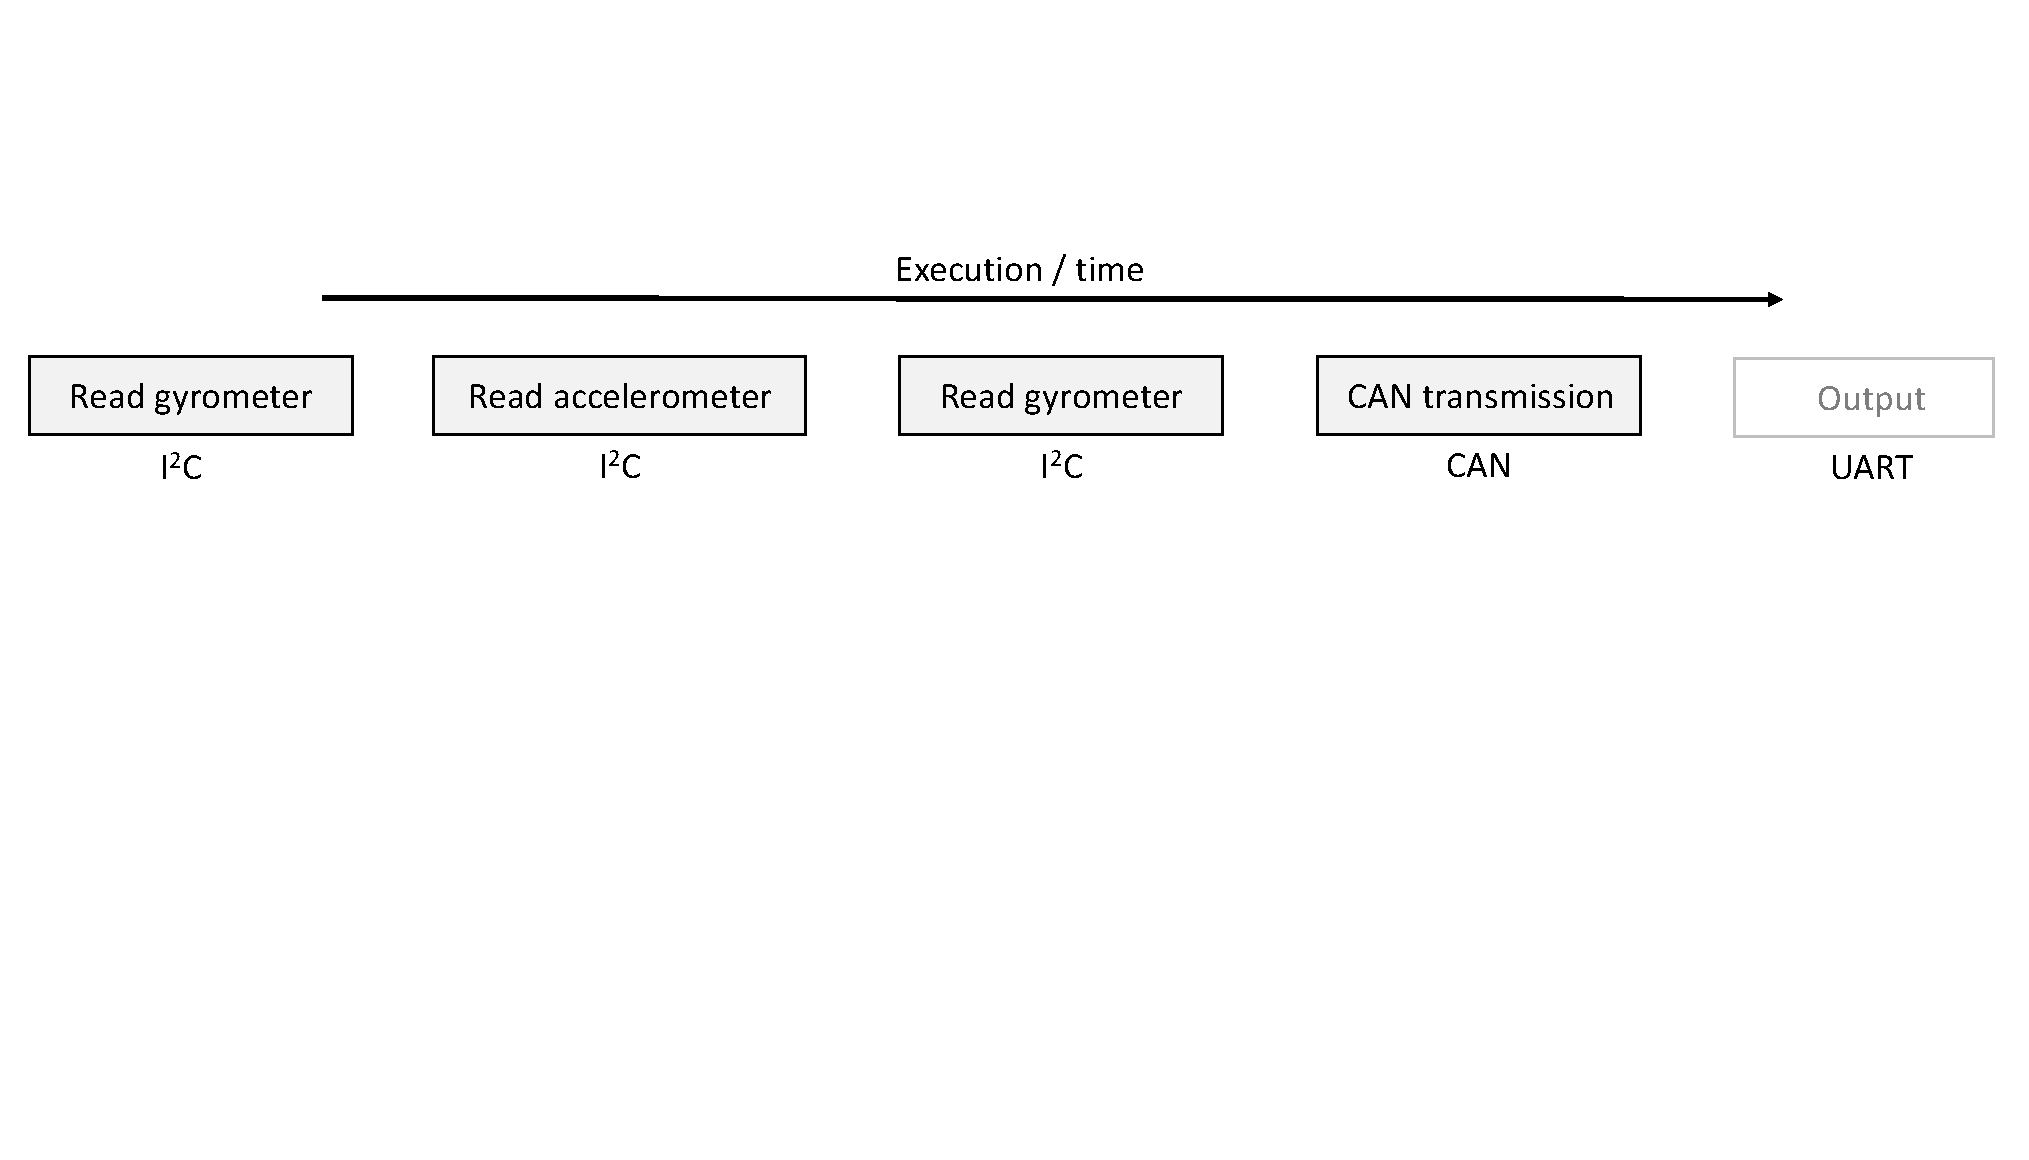
\includegraphics[width=1\linewidth]{figures/arduino_delays_sketch}
\caption{Execution blocks for IMU data acquisition on the Arduino Due (overview)}
\label{fig:arduino_delays_sketch}
\end{figure*}


\section{Vehicle testing}
\label{sec:vehicle-testing}

\subsection{System calibration}
\subsection{Actuator tests}
\subsection{Algorithm evaluation}
\subsection{Sensor testing}

\begin{itemize}
	\item test angle sensor offline
	\item zero IMUs, make sure paired sensors show the same outputs
	
\end{itemize}

\section{Hardware-in-the-loop testing}
\label{sec:HIL}
\begin{itemize}
	\item description of HIL
	\item Functional architecture diagram (MSD replaced with actual dolly)
	\item Limitations (axle loads, standing still)
\end{itemize}

Usually a hardware iLack in processing power does not allow for VTM's execution in the dSpace environment on the MABII. To perform HIL-test it was thus necessary to split the comptuation and allow for real-time data exchange between the hardware controlling system on the MABII and the rest of the simulation which will run on a standard PC. 

\begin{figure*}[h]
\centering
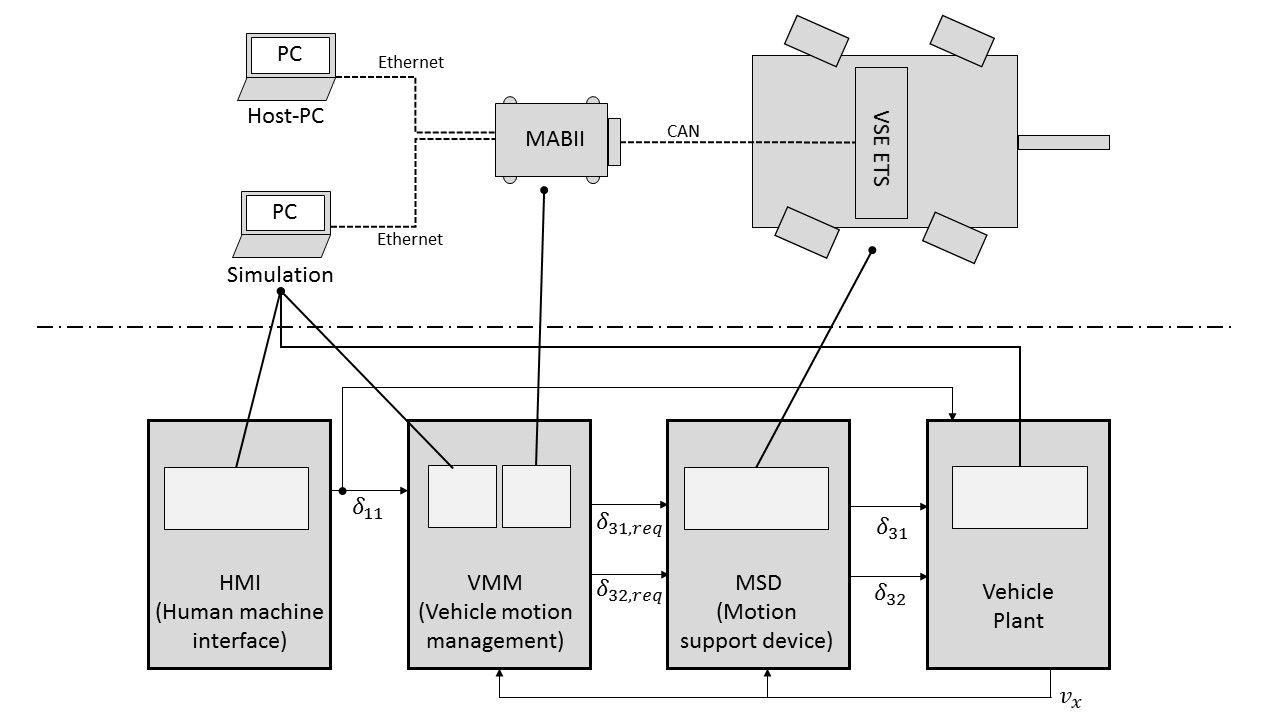
\includegraphics[width=1\linewidth]{figures/HIL_overview}
\caption{Overview of HIL-simulation, distribution of sub-functions over different physical platforms (top) and correlation to Volvo functional architecture (bottom)}

\label{fig:HIL_overview}
\end{figure*}


\subsection{Low-speed controller}
\subsection{High-speed controller}

\section{Track testing}
\label{sec:track-testing}

\subsection{Testmaneuvers}

\begin{itemize}
	\item lit research for standard maneuvers
	\item sine-wave
	\item outline critical parts of maneuver
	\item figure with SA over time
	\item expected behaviour from simulation
\end{itemize}

\subsection{Testenvironment AstaZero}

\begin{itemize}
	\item overview of AZ
	\item map in appendix?
	\item restrictions of environment
	
\end{itemize}

\subsection{Testmatrix}

\begin{itemize}
	\item checklist for launch
	\item parameters that very varied
	\item different runs
	\item planned maneuvers
	
\end{itemize}

\subsection{Test setup and instrumentation}

\begin{itemize}
	\item detailed description of placement of sensors, wiring, logging-PC
\end{itemize}


\end{document}
